\section{Dataset Preparation}

Two albums for each artist were selected based off similar musical styles and vocal features. These were 

Following the selection of the 2 albums for each artist and removal of any songs where additional vocal artists to the main vocalist featured were removed, all songs were passed through the Spleeter model\cite{SpleeterPip}\cite{SpleeterPip}. The model outputted 2 seperate tracks for each song, one representing instrumentals and one vocals. The instrumental tracks were discarded.

\begin{figure}
    \centering
    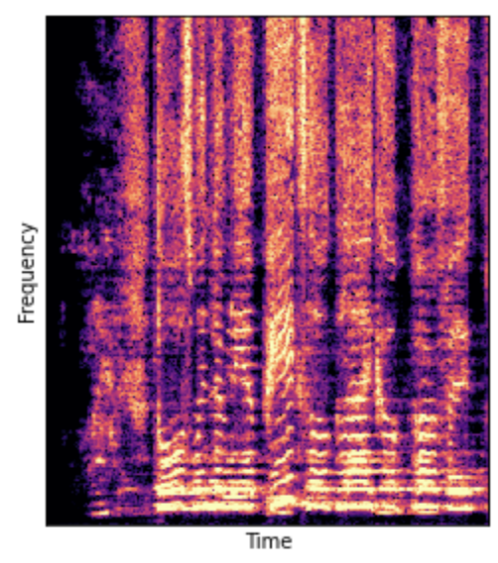
\includegraphics[width=0.6\textwidth]{research/PreprocessingSpecplot.png}
    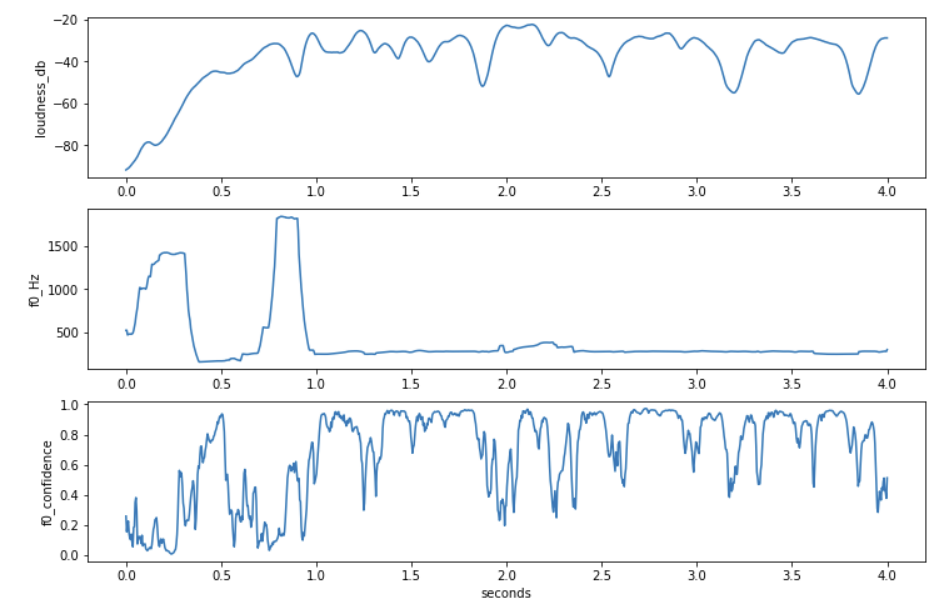
\includegraphics[width=0.8\textwidth]{research/PreprocessingFeatures.png}
    \caption{Dataset Preprocessing: Spectrogram plot of a random 4 second sample from one of the datasets and its accomanying F0, F0 Confidence and Amplitude characteristics over time throughout the sample}
\end{figure}

Preprocessing of the datasets involved spliting the raw audio into smaller samples each 4 seconds long. For each sample F0 and confidence of F0 probability was inferred using CREPE\cite{CREPE}. Amplitude was computed statistically using the Librosa library\cite{LibrosaPip}. The 4 second samples and accomanying features were then stored as TFRecord files.

Each of the 2 datasets were preprocessed on Google Colab notebooks, this process took approximately 40 minutes for each dataset using a NVIDIA Tesla V100 GPU.

Finally, from each dataset a random 4 second clip was selected to prove successful preprocessing. Its its spectrogram was computed and plotted. Computed F0, F0 Confidence and Amplitude characteristics were also plotted for the selected clip. The udnerlying audio sample could also be played.